\section{Introduction}\label{sec:intro}

A system that rewrites its own weights, its own code or its own proofs, and keeps a rewrite when a test passes, is the basic unit of every proposal for recursive self-improvement. Good described the end point in 1965: a machine that designs a better machine, which designs a better one still, in an ``intelligence explosion'' that leaves human intelligence far behind \cite{Goo66}.\footnote{I.~J. Good, \emph{Speculations concerning the first ultraintelligent machine}, written in 1965 and printed in Advances in Computers, volume~6 (1966), pages 31--88 \cite{Goo66}. Good's argument is that an ultraintelligent machine could design better machines, so the first such machine is ``the last invention that man need ever make, provided that the machine is docile enough to tell us how to keep it under control''. The proviso is the subject of the present paper in a precise form: the docility we ask for is that every improvement the machine keeps has been checked, and we compute what the checking costs.} The literature since then has asked mostly how fast such a process could grow, under which assumptions on the returns to intelligence it reaches a vertical asymptote, and which physical limits stop it \cite{Ord26,AOA25}. We ask a different question, which has a sharper answer: what does it cost to make sure that what the process keeps is correct?

A second question sits beside the first. A language model proposes, and a measurement on $11{,}683$ research papers shows how its proposals differ from those of the people who wrote the papers: the ideas of every model tested crowd into one or two kinds, chiefly the transfer of a method from one field to another, while human authors spread theirs over gaps in the evidence, mismatched scope and unexplained puzzles \cite{CZC26}. A sound system whose proposer seldom reaches the kind of idea a problem needs is sound and slow. We price this second gap with the same tools as the first, prove the least number of proposals any proposer can reach, measure how far the models are from it, and build a selector that learns from the checks alone to close it.

We call the object a \emph{BLLM}, a system beyond the language model. It has three parts (Fig.~\ref{fig:architecture}). A generator, which may be a large language model \cite{VSP17,BMR20}, proposes candidate modifications of the system. A bank of randomized checks tests each candidate; a check has perfect completeness, so a correct candidate always passes, and soundness $\eps<1$, so an incorrect candidate passes one run with probability at most $\eps$. A memory keeps a candidate only after it has passed every run allotted to it, and the generator works from the memory. The name and the loop come from the verifier-gated engine of \cite{Bha26a}, in which a generator proposes steps toward a proof and a verifier accepts or rejects each one; we replace the single verifier by a schedule of independent runs, and that replacement is what makes the cost of soundness computable. The checks are the learned verifiers of \cite{CKB21,UKK22,LKB23}, the randomized identity tests of \cite{Sch80,Zip79}, the interactive and probabilistically checkable proofs of \cite{GMR89,Bab85,AS98,ALM98}, or a proof checker such as Lean \cite{MU21} run on a randomized search. The cost of a run of the check of the $i$-th candidate is $a_{i}>0$, and the schedule gives that check $r_{i}$ independent runs.

\begin{figure*}[t]
\centering
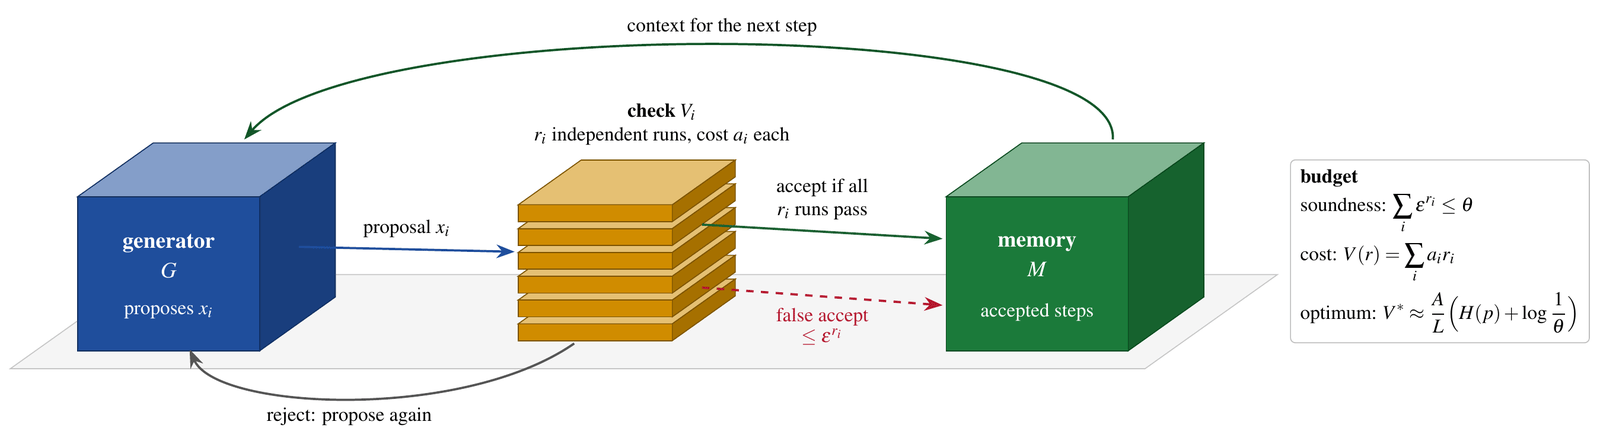
\includegraphics[width=0.94\textwidth]{figures/fig_architecture}
\Description{Block diagram: a generator sends candidate modifications to a bank of checks; accepted candidates enter the system and the cost of all runs is charged to one budget.}
\caption{A BLLM. The generator proposes candidate modifications; the $i$-th candidate is tested by $r_{i}$ independent runs of a check $V_{i}$ of cost $a_{i}$ per run; an incorrect candidate survives all runs with probability at most $\eps^{r_{i}}$ and a correct one always survives; the memory keeps what survives and feeds it back as context. The budget box states the two quantities the paper controls, the expected number of false acceptances $\sum_{i}\eps^{r_{i}}\le\theta$ and the cost $V(r)=\sum_{i}a_{i}r_{i}$, and the value of the optimum (Theorem~\ref{thm:A}).}
\label{fig:architecture}
\end{figure*}

\subsection{What the title means}

The title names two properties, and each is a measured quantity of the system we built, which we call Anaxia (Section~\ref{sec:network}).

\emph{Beyond the LLM} means that a language model, where one is used at all, only proposes. Whether a proposal is kept is decided by checks whose error is priced by the laws of this paper, and every object that the engine keeps from a search is checked again by code that shares nothing with the search. A language model that writes an answer and grades it with the same weights is the case these laws exclude: its check is not independent of its proposal, so the runs of the model have no soundness to spend.

\emph{Deep Human-Mind-AI} means three things, each of which we measure and none of which says that the engine thinks as a person does.
\begin{enumerate}[label=(\alph*),leftmargin=1.8em,itemsep=1pt]
\item \emph{Proposals distributed as people distribute them.} On the axis of research opportunities of \cite{CZC26} the least expected number of proposals per problem is $6.50$; the profile of the human authors pays $7.00$, a factor $1.08$, and the nine language models measured pay between $1.51$ and $4.28$ times the optimum (Table~\ref{tab:gap}). The selector of the engine learns the profile that attains the optimum from the results its checks keep.
\item \emph{Human constructions as the raw material.} The default proposer is not a model but a typed crossing of constructions that mathematicians wrote down, each kept with its provenance, its type and the types it needs, so that a new candidate is a composite of known pieces that fit.
\item \emph{Construction by hand, mechanised.} Construction mode writes down a new object together with the argument for what it forces, as a combinatorialist builds a gadget, and keeps it only after an independent check. From the rules of Steinberg's problem alone it rebuilt the gadgets of the counterexample of Cohen-Addad, Hebdige, Kr\'al', Li and Salgado \cite{CHK17}.
\end{enumerate}

\subsection{The entropy law}

Write $A=\sum_{i}a_{i}$ for the total cost of one run of every check, $p_{i}=a_{i}/A$ for the cost profile, $H(p)=\sum_{i}p_{i}\log(1/p_{i})$ for its entropy, and $L=\log(1/\eps)$. The schedule $r$ is \emph{$\theta$-sound} when the expected number of incorrect candidates kept is at most $\theta$ in every assignment of correct and incorrect candidates, which for checks whose soundness $\eps$ is attained is the inequality $\sum_{i}\eps^{r_{i}}\le\theta$ (Section~\ref{sec:model}). Its cost is $V(r)=\sum_{i}a_{i}r_{i}$, the cost of certifying a run in which every candidate is correct, and $\Vs(\theta)$ is the least cost of a $\theta$-sound schedule.

\begin{mainthm}[Entropy law]\label{thm:A}
For $0<\theta\le1$,
\begin{equation}\label{eq:entropylaw}
\frac{A}{L}\Bigl(H(p)+\log\frac1\theta\Bigr)\ \le\ \Vs(\theta)\ \le\ \frac{A}{L}\Bigl(H(p)+\log\frac1\theta\Bigr)+A .
\end{equation}
The lower bound is attained when every $\theta p_{i}$ is an integer power of $\eps$, and the additive constant $A$ cannot be replaced by $cA$ with $c<1$. The same bounds hold for infinitely many candidates with $A<\infty$, and for schedules drawn at random independently of the checks.
\end{mainthm}

The law says that the price of soundness is an entropy. Certifying $n$ candidates of equal cost costs $(n/L)\log(n/\theta)$ up to $n$, so the tax per candidate grows like $\log n$ and not like a constant: a system that keeps more modifications must test each one harder. A skewed profile is cheaper than a flat one with the same total, because the expensive checks may be run fewer times and the cheap ones more, and the saving is measured exactly by $\log n-H(p)$. The schedule that attains the bound runs the $i$-th check $\lceil\log(A/(\theta a_{i}))/L\rceil$ times, so it spends $\log(1/p_{i})$ nats of soundness on a candidate of relative cost $p_{i}$: this is Shannon's code length \cite{Sha48}, and the analogy is exact.

\begin{mainthm}[Huffman schedules]\label{thm:C}
If $\eps=1/D$ for an integer $D\ge2$ and $\theta=D^{-k}$ for an integer $k\ge0$, then the $\theta$-sound schedules are exactly $r_{i}=\ell_{i}+k$ with $(\ell_{i})$ the lengths of a $D$-ary prefix code, and $\Vs(\theta)=A\bigl(k+L_{D}(p)\bigr)$, where $L_{D}(p)$ is the expected length of a Huffman code for $p$.
\end{mainthm}

So the optimal schedule is computed by Huffman's algorithm \cite{Huf52}, and Kraft's inequality \cite{Kra49,McM56} is the soundness condition in disguise. The additive constant of Theorem~\ref{thm:A} is the redundancy of the Huffman code, which lies in $[0,1)$ in units of $\log D$ \cite{CT06,Gal78}.

Not every check is repeated. A statistical check that averages $m$ samples and accepts when the average is close to its target has false acceptance probability of order $1/m$ by Chebyshev's inequality, not $\eps^{m}$. For a check whose cost to reach false acceptance probability $\delta$ is $a\delta^{-s}$ the entropy is replaced by a R\'enyi entropy \cite{Ren61}.

\begin{mainthm}[R\'enyi law]\label{thm:D}
For checks of polynomial order $s>0$ and $0<\theta\le1$, the least cost of a $\theta$-sound allocation is
\begin{equation}\label{eq:renyilaw}
\Vs_{s}(\theta)=\theta^{-s}\Bigl(\sum_{i}a_{i}^{1/(1+s)}\Bigr)^{1+s}=A\,\theta^{-s}e^{sH_{\alpha}(p)},
\end{equation}
where $\alpha=1/(1+s)$ and $H_{\alpha}$ is the R\'enyi entropy of order $\alpha$; and $\Vs_{s}(\theta)=A\bigl(1+s(H(p)+\log\frac1\theta)\bigr)+O(s^{2})$ as $s\to0$.
\end{mainthm}

The first-order term at $s=0$ is the entropy law, so the R\'enyi law is a one-parameter deformation of it, as Campbell's coding theorem is a deformation of Shannon's \cite{Cam65}. Section~\ref{sec:renyi} also gives a criterion, valid for every cost function, for an infinite sequence of candidates to admit a sound schedule of finite cost.

\subsection{Chains, gates and singularities}

Section~\ref{sec:chains} puts the checks into a self-improvement chain in which the generator retries a step until a candidate is kept. When each step is wrong with probability between $\rho_{\ast}>0$ and $\bar\rho<1$, the least expected cost of the chain with at most $\theta$ expected false acceptances is pinched between the entropy law at budget $\theta/\rho_{\ast}$ and the entropy law at budget $\theta(1-\bar\rho)/\bar\rho$, divided by $1-\bar\rho$ (Theorem~\ref{thm:B}). The same section proves an exponential separation between checking every step and checking only the outcome: with perfect checks the ratio of expected costs is $(1-\rho)^{-(n-1)}\ge e^{(n-1)\rho}$, and with imperfect checks the step check may accept an incorrect step with probability of order $1/n$ while the outcome check must do so with probability exponentially small in $n$ (Theorem~\ref{thm:gating}).

An infinite chain whose total expected cost is finite completes infinitely many improvements in finite cost, and we call it \emph{singular}, after the vertical asymptote of the explosion literature. It is \emph{sound} when the number $F$ of incorrect modifications it keeps is finite.

\begin{mainthm}[Sound singularities]\label{thm:E}
Let the $n$-th step cost $g_{n}$ to generate and $a_{n}\le1$ per run to check, with error probabilities in $[\rho_{\ast},\bar\rho]\subset(0,1)$, independent steps and checks of exact soundness $\eps$. Then
\begin{enumerate}[label=\textup{(\roman*)},leftmargin=2.2em,itemsep=1pt]
\item $F<\infty$ almost surely, or $\PR(F=0)>0$, if and only if $\sum_{n}\eps^{r_{n}}<\infty$, and otherwise $F=\infty$ almost surely;
\item a singular chain in which every step is checked exists if and only if $\sum_{n}g_{n}<\infty$ and $\sum_{n}a_{n}<\infty$;
\item a sound singular chain exists if and only if in addition $\sum_{n}a_{n}\log(1/a_{n})<\infty$.
\end{enumerate}
\end{mainthm}

So there is a soundness gap. For $a_{n}=1/(n\log^{\beta}n)$ a singular chain exists for every $\beta>1$, and a sound one only for $\beta>2$; between the two, every schedule fast enough to reach the asymptote keeps infinitely many errors almost surely (Corollary~\ref{cor:gap}). For a power law $a_{n}=n^{-p}$ the price of soundness, the ratio of the cheapest sound cost to the cost of one run per step, is $1/((p-1)L)+O(\log\frac1{p-1})$, and with polynomial checks of order $s$ a sound singularity exists exactly when $p>1+s$ (Fig.~\ref{fig:regimes}).

When the improvements branch, each kept improvement spawning a random number of candidates, the process is a Galton--Watson tree \cite{WG75,AN72}.

\begin{mainthm}[Branching takeoff]\label{thm:F}
Let $m$ be the mean number of correct offspring kept per kept improvement, and let the check of generation $k$ accept an incorrect candidate with probability $\delta_{k}$. Then the takeoff survives with positive probability if and only if $m>1$; the expected number of kept errors is $\mu(1-\gamma)\sum_{k\ge1}m^{k-1}\delta_{k}$; and if this series diverges then, under $\EE\,\xi\log\xi<\infty$, infinitely many errors are kept almost surely on survival. With exponential checks, soundness forces $r_{k}\ge k\log m/L$ for all large $k$, and $r_{k}=\lceil k\log(2m)/L\rceil$ suffices.
\end{mainthm}

Here $\mu$ is the mean number of candidates per kept improvement, $\gamma$ the probability that a candidate is correct and $\xi$ the number of candidates. A fixed false acceptance rate, however small, is fatal to an explosive takeoff, and the number of runs per check must grow linearly in the generation, that is, logarithmically in the size of the population: the entropy tax again.

\subsection{Without foresight, among many agents}

The schedules above are computed from the whole cost profile. A system that improves itself does not know its future candidates: when the $n$-th one arrives, only $a_{1},\dots,a_{n}$ are known, and the runs of its check must be fixed then. Theorem~\ref{thm:G} gives a rule that uses only the running total $S_{n}=a_{1}+\dots+a_{n}$, is $\theta$-sound for every sequence of costs, and pays over the offline optimum at most $\frac{A_{N}}{L}\bigl(\log2+2\log(1+\log\frac{A_{N}}{a_{1}})\bigr)+A_{N}$ on the first $N$ candidates; on the doubling costs every online rule pays an excess of order $\frac{A_{N}}{L}\log\log\frac{A_{N}}{a_{1}}$, so the double logarithm is the true price of not knowing the future (Fig.~\ref{fig:online}). Consequently the criterion of Theorem~\ref{thm:E} needs no oracle: a chain that knows only its past reaches a sound singularity whenever any chain does (Corollary~\ref{cor:onlinesing}).

A working system also delegates. When a coordinator splits the candidates among subagents, the entropy satisfies the chain rule over the split, and Theorem~\ref{thm:H} shows that a coordinator which gives each subagent the share of the budget proportional to its total cost loses nothing: each subagent, knowing only its own costs and one number, computes on its candidates exactly the optimal schedule of the whole system, and along a tree of delegation the entropy tax is paid node by node. Any other split costs exactly $\frac AL$ times a Kullback--Leibler divergence. Finally, cheap checks of soundness $\eps$ placed before one exact check of cost $c$ make the exact check paid only on the correct candidates, with a premium $\frac bL(1+\log\frac{c\rho L}{b})$ logarithmic in the ratio of costs (Theorem~\ref{thm:cascade}). These two results are the laws of the system of subagents built in Section~\ref{sec:agents}; Appendix~\ref{sec:cases} reads six machine-checked or published proofs of hard problems in their terms.

\subsection{The gap between human and LLM thinking}

Let a problem need an idea of class $j$ with probability $\pi_{j}$, and let a proposer draw classes from a profile $q$ until it draws the needed one. The expected number of proposals is $\sum_{j}\pi_{j}/q_{j}$, and Theorem~\ref{thm:I} shows that it is at least $e^{H_{1/2}(\pi)}=(\sum_{j}\sqrt{\pi_{j}})^{2}$, a R\'enyi entropy of order one half, attained only by square-root sampling; the excess is exactly $e^{H_{1/2}(\pi)}$ times the chi-squared divergence of $q$ from square-root sampling, and mixing a fraction $\lambda$ of square-root sampling into any proposer brings its cost under $e^{H_{1/2}(\pi)}/\lambda$. On the data of \cite{CZC26} the optimum is $6.50$ proposals per problem on the axis of research opportunities and $6.45$ on the axis of methods; the human profile itself pays $7.00$, and the nine models pay from $1.51$ to $4.28$ times the optimum (Table~\ref{tab:gap}). A BLLM learns the need from the results its checks keep, and its excess over the optimum falls like $\beta(\pi)/(4n)$ after $n$ closed problems (Proposition~\ref{prop:learnrate}), for a constant $\beta(\pi)$ that is $7.06$ on the human profile of opportunities. The learning is done by a race of leaky integrate-and-fire neurons with a reward-modulated synapse, which samples exactly the square root of the counts it has learned (Proposition~\ref{prop:spiking}). Appendix~\ref{sec:brains} sets this circuit beside three wiring diagrams measured synapse by synapse, of the worm \textit{C.~elegans}, of the fly \textit{Drosophila} and of a cubic millimetre of human cortex, and computes from them the sensory-to-motor depth, the modular structure and the laminar composition that the three parts of a BLLM reproduce.

\subsection{Towers}

An engine can act on another engine: one that chooses among strategies of a proposer and keeps the strategies that work stands on the proposer, and one that runs several copies of it and keeps the better half stands on that. Section~\ref{sec:towers} prices such a tower. If $n$ verified layers share a budget $\theta$ of false acceptances, because a false acceptance low in the tower contaminates everything above it, then certifying the tower costs at least $n\log(n/\theta)$ nats of soundness, each added layer raises the bound by at least $\log((n+1)/\theta)$, and past a finite depth every tower costs more than any fixed amount (Theorem~\ref{thm:tower}). Depth pays only while it lowers the search by more than the increment, and the theorem says that this stops.

\subsection{The engine and what it did}

The theorems price the checks; they do not say where good candidates come from. Section~\ref{sec:network} describes the engine and Sections~\ref{sec:experiments} to~\ref{sec:hodgeround} measure it. Known constructions are typed nodes, each with the type of object it gives and the types it needs; a candidate is a cross that fills an input of one construction with the output of another; every closed cross is checked by a program, attacked by a refuter, and recorded in a shared memory. A target point fixes for each problem the statement that would settle it, five agents, one per problem, attack through a channel that brings every relevant record of the memory to the proposer, and construction mode builds new objects where crossing has nothing to combine. We ran the engine on five open problems, the lattice mass gap of Yang--Mills theory, the Hodge conjecture, Grothendieck's standard conjecture of Lefschetz type, Chowla's conjecture and Erd\H{o}s problem 1183, on Steinberg's problem as a calibration, and on two conjectures from mathematical physics. The measurements are these.
\begin{enumerate}[label=(\roman*),leftmargin=1.8em,itemsep=1pt]
\item \emph{Typing does the work.} On Yang--Mills the network reached in every run a composite whose check accepts a lattice mass gap for four-dimensional $\mathrm{SU}(2)$ on $\beta_{W}<\frac13$, which no run of random or type-filtered pairing reached; random pairing wastes $45$ of $48$ crosses on ill-typed pairs. The composite was first proposed by the language-model proposer and then entered in the library, so the network reproduces the step rather than originating it. The step itself, Theorem~\ref{thm:onethird}, is proved here and has not been refereed; it extends the range $\beta_{W}<\frac29$ of \cite{BB26d}, and Proposition~\ref{prop:forestceiling} shows that $\frac13$ is the ceiling of the method.
\item \emph{Boosters do not help.} Hebbian weights with path credit reached that step in $12$ and $14$ of $200$ runs against $21$ for the unboosted network, a difference within two standard errors; a booster strengthens synapses that have fired, and the step needed one that had not.
\item \emph{Memory halves the cost.} Over $60$ seeds and five rounds the full system reaches its plateau of about six survivors with $46.4$ checks against $95.2$ without memory, because it never checks a decided composite twice; it does not raise the plateau.
\item \emph{Agents are cheaper and reach no further.} After eleven rounds the five agents hold $24$ distinct survivors for $250$ checks and a single loop $27$ for $797$; the agents level off in the second round, the loop passes them in the sixth with known results, and no survivor of either reaches a target point.
\item \emph{Patterns transfer partially or fail.} Of $38$ transfers of a pattern that broke a comparable barrier elsewhere to a blocking step, none closes, $7$ give a weaker statement or a new computation and $31$ fail, for one of three reasons recorded in Section~\ref{ssec:matrix}.
\item \emph{Construction mode rebuilds what crossing cannot.} Random planar frames filled with library gadgets gave no gadget of Steinberg's kind in $2.45$ million frames; the goal-directed builder, given only the rules, rebuilt the $15$-vertex gadget of \cite{CHK17} on its $116$th try after $11$ seconds. With that gadget and a triangle as lemmas it built a $42$-vertex gadget with the contacts of the second gadget of \cite{CHK17} on two seeds, and on a third a $48$-vertex gadget with contact distances $5,4,5$, which \cite{CHK17} does not use, and the assembly of \cite{CHK17} applied to the rebuilt $15$-vertex gadget gives a planar graph of $166$ vertices with no cycle of length $4$ or $5$ that three satisfiability solvers find not $3$-colourable. On Erd\H{o}s's question, which also forbids cycles of length $6$, it finds nothing (Section~\ref{ssec:steinberg}).
\item \emph{Depth pays once.} At equal budgets of exact checks, a second layer that first builds an easier gadget and keeps it as a lemma reaches the profile of the second gadget of \cite{CHK17} on seven of ten runs, where the builder alone never reaches it; a third layer reaches it on six. When all layers share one library and one set of weights, the step from the lemma to the goal takes a median of $308$ checks against $2{,}342$ when each copy keeps its own. The crossing loop, given $13$ to $20$ times the budget, finds no gadget, and no tower finds one on Erd\H{o}s's question (Section~\ref{ssec:towerbench}).
\item \emph{One problem only.} Pointed at the Hodge conjecture alone, with every result of \cite{BB26c} and of the companion paper \cite{BMB26b} in its library, the engine excludes by counting two of the configurations left open on $E_{0}^{6}$, a parity count on the closed chains against the Chern character excludes a third up to seven line bundles at every discriminant, the fourth reduces to the ranks of explicit Massey products, and the gap of every target point is the same after the last round as after the first (Section~\ref{sec:hodgeround}).
\item \emph{It learns from its failures.} Every failed attempt writes a record that names the part that failed, changes one rule of the engine and is closed by the outcome of the next attempt under the changed rule. In the log so far, \modChanges{} changes of rule followed \modAttempts{} attempts on \modTargets{} targets, and of the \modBuilt{} changes that were built, \modRetryClosed{} led to a retry that closed its target and \modRetryPartial{} more to one that moved it forward. The loop never makes the same change twice on a target, so it stops after at most one attempt more than there are changes it can propose (Proposition~\ref{prop:loopstops}), and it ranks the kinds of change by the posterior mean of their success (Proposition~\ref{prop:playbook}); Section~\ref{sec:selfmod}.
\item \emph{A benchmark crossed.} On a conjecture about the reflexive polytopes of dimension four, whose Calabi--Yau hypersurfaces form the largest known list of Calabi--Yau threefolds, the engine reached a proof: shrunk one reflexive polytope at a time, such a polytope reaches a seed in at most $\seedBound$ steps, for all $\seedCount$ polytopes of the Kreuzer--Skarke list, because each step lowers the number of lattice points of the polytope and raises that of its dual (Theorem~\ref{thm:seedbound}). In dimensions two and three the sharp constants are $\seedTwo$ and $\seedThree$; in dimension four the sharp constant lies between $\seedLow$ and $\seedBound$ and is open. This passes the sixth benchmark, one open conjecture of mathematical physics proved without conditions (Section~\ref{sec:seed}).
\end{enumerate}
On Erd\H{o}s problem 1183 a reduction to weighted posets (Lemma~\ref{lem:levelposet}) gives the upper bounds that, with the known lower bounds, determine $f(n)$ for $n\le20$ (Theorem~\ref{thm:fvalues}). None of the five problems is solved, and Section~\ref{ssec:whyhard} states for each the step at which every construction we hold stops; the sixth benchmark is passed, by the seed conjecture.

\subsection{What the paper proves}

Table~\ref{tab:results} lists the results. The proofs are complete and elementary: the entropy law rests on the inequality $\log x\le x-1$, the R\'enyi law on H\"older's inequality, the singularity theorem on the Borel--Cantelli lemmas, the online law on a telescoping inequality for $\log(S_{n}/a_{1})$, the branching theorem on the Kesten--Stigum theorem \cite{KS66} and L\'evy's conditional form of the Borel--Cantelli lemma \cite{Dur19}, and the tower law on the entropy law with unit costs. Every finite inequality, the online and subagent laws, the gap law, the cascade bounds, the Kraft--schedule correspondence, the R\'enyi optimum, the convergence criteria for sound schedules, both Borel--Cantelli statements and the tower law are proved in Lean~4 with Mathlib, in sixty-five theorems that depend only on the three standard axioms (Appendix~\ref{app:checks}); the probabilistic limit theorems and the asymptotics of the zeta function are proved in the text and are not formalised.

The paper does not prove that any existing system is sound, and it does not predict whether an intelligence explosion will happen. Its theorems are conditional on a model, stated in Section~\ref{sec:model}: independent runs, perfect completeness, and schedules fixed in advance. Remark~\ref{rem:adaptive} shows that the last assumption matters, since a schedule allowed to stop at the first detected error escapes the entropy term at the price of discarding good work. What the paper does establish is that, inside the model, the cost of soundness is computable in closed form, that it is an entropy, and that it separates the singular processes into sound and unsound ones by a single convergent series.

\begin{table*}[t]
\caption{The main results. $A=\sum a_{i}$, $p=a/A$, $L=\log(1/\eps)$; ``Lean'' names the formalised statements of Appendix~\ref{app:checks}.}
\label{tab:results}
\centering
\footnotesize
\setlength{\tabcolsep}{4pt}
\begin{tabular}{@{}p{0.13\textwidth}p{0.36\textwidth}p{0.13\textwidth}p{0.32\textwidth}@{}}
\toprule
\rr Result & \rr Statement & \rr Proof & \rr Lean \\
\midrule
\rr Theorem~\ref{thm:A} & \rr $\frac AL(H+\log\frac1\theta)\le \Vs(\theta)\le \frac AL(H+\log\frac1\theta)+A$ & \rr Gibbs, ceilings & \rr \lean{verification\_lower}, \lean{ceilSchedule\_cost} \\
\rr Proposition~\ref{prop:clean} & \rr clean runs: budgets $\theta$ and $\log\frac1{1-\theta}$ & \rr $1-\sum q\le\prod(1-q)\le e^{-\sum q}$ & \rr \lean{clean\_ge}, \lean{clean\_budget} \\
\rr Proposition~\ref{prop:random} & \rr random oblivious schedules obey Theorem~\ref{thm:A} & \rr Jensen & \rr \lean{randomised\_budget} \\
\rr Proposition~\ref{prop:twosided} & \rr two-sided checks, rate $\frac12\log\frac1{4q(1-q)}$ & \rr Chernoff & \rr --- \\
\rr Theorem~\ref{thm:C} & \rr $\Vs(D^{-k})=A(k+L_{D}(p))$ & \rr Kraft, Huffman & \rr \lean{kraft\_of\_schedule}, \lean{schedule\_of\_kraft} \\
\rr Theorem~\ref{thm:D} & \rr $\Vs_{s}(\theta)=A\theta^{-s}e^{sH_{1/(1+s)}(p)}$ & \rr H\"older & \rr \lean{renyi\_lower}, \lean{renyi\_attain} \\
\rr Theorem~\ref{thm:dual} & \rr sound schedule $\iff\sum a_{n}\psi(\lambda/a_{n})<\infty$ & \rr Legendre duality & \rr \lean{schedule\_of\_dual\_summable} \\
\rr Theorem~\ref{thm:B} & \rr chain cost between two entropy laws & \rr Wald & \rr \lean{entropy\_lower}, \lean{ceilSchedule\_sound} \\
\rr Theorem~\ref{thm:gating} & \rr step versus outcome checks: $(1-\rho)^{-(n-1)}$ & \rr products & \rr \lean{separation}, \lean{precision\_bounds} \\
\rr Theorem~\ref{thm:E} & \rr sound singularity $\iff\sum g,\sum a,\sum a\log\frac1a<\infty$ & \rr Borel--Cantelli & \rr \lean{sound\_schedule\_iff}, \lean{false\_accepts\_infinite} \\
\rr Corollary~\ref{cor:gap} & \rr soundness gap $1<\beta\le2$ & \rr condensation & \rr --- \\
\rr Proposition~\ref{prop:powerlaw} & \rr price $\sim1/((p-1)L)$ for $a_{n}=n^{-p}$ & \rr integral comparison & \rr --- \\
\rr Proposition~\ref{prop:osgood} & \rr Osgood takeoff: check time $\asymp\kappa/(c(\alpha-1)^{2}L)$ & \rr entropy of $\zeta$ & \rr --- \\
\rr Theorem~\ref{thm:G} & \rr online rule: excess $\le\frac{A_{N}}L(\log2+2\log(1+\log\frac{A_{N}}{a_{1}}))+A_{N}$ & \rr telescoping & \rr \lean{onlineSchedule\_sound}, \lean{online\_lower} \\
\rr Theorem~\ref{thm:H} & \rr split price $\frac AL(D(P\|q)+\log\frac\theta\Theta)$ & \rr chain rule & \rr \lean{chain\_rule}, \lean{split\_lower}, \lean{proportional\_split} \\
\rr Theorem~\ref{thm:cascade} & \rr cascade: $\min E=c(1-\rho)+\frac bL(1+\log\frac{c\rho L}b)+O(b)$ & \rr $\log x\le x-1$ & \rr \lean{cascade\_lower}, \lean{cascade\_upper} \\
\rr Theorem~\ref{thm:F} & \rr branching takeoff and $r_{k}\ge k\log m/L$ & \rr Kesten--Stigum, L\'evy & \rr \lean{amplified\_summable}, \lean{contamination\_diverges} \\
\rr Theorem~\ref{thm:tower} & \rr $n$ layers: $\sum_{k}\log\frac1{\beta_{k}}\ge n\log\frac n\theta$; saturation & \rr Theorem~\ref{thm:A}, unit costs & \rr \lean{tower\_cost\_lower}, \lean{tower\_saturates} \\
\rr Theorem~\ref{thm:I} & \rr proposals $\sum\pi_{j}/q_{j}\ge e^{H_{1/2}(\pi)}$, excess $e^{H_{1/2}}\chi^{2}(r\|q)$ & \rr Cauchy--Schwarz & \rr \lean{search\_lower}, \lean{search\_chi2}, \lean{search\_mix} \\
\rr Proposition~\ref{prop:learnrate} & \rr learned square-root sampling: $1+\beta(\pi)/(4n)$ & \rr second-order expansion & \rr --- \\
\rr Proposition~\ref{prop:spiking} & \rr first spike of the race is $\sqrt{c_{k}+\alpha}/\sum_{l}\sqrt{c_{l}+\alpha}$ & \rr exponential race & \rr --- \\
\rr Lemma~\ref{lem:depth} & \rr processing depth of a wiring diagram & \rr Laplacian & \rr --- \\
\bottomrule
\end{tabular}
\end{table*}

\subsection{Organisation}

Section~\ref{sec:history} traces the lines that meet here: self-reference and the intelligence explosion, coding and testing, branching processes, and verifiers for language models; Section~\ref{sec:related} sets the engine beside the systems that search against an evaluator, FunSearch, AlphaEvolve, AlphaProof and the provers trained against Lean, and says what is taken from each and what is not. Section~\ref{sec:model} defines the model. Sections~\ref{sec:entropy} to~\ref{sec:renyi} prove the entropy law, its Huffman form and its R\'enyi deformation. Section~\ref{sec:chains} treats chains and the comparison of step and outcome checks, Section~\ref{sec:singularity} singular chains, Section~\ref{sec:online} the online law, Section~\ref{sec:agents} subagents and cascades, Section~\ref{sec:gap} the gap between human and model proposals and the spiking selector that closes it, Section~\ref{sec:branching} the branching takeoff and Section~\ref{sec:towers} towers of verified layers. Section~\ref{sec:network} describes Anaxia, Section~\ref{sec:benchmark} the six benchmarks with their pass lines, Section~\ref{sec:experiments} the measurements of the crossing network, Section~\ref{sec:construct} construction mode and the towers at equal cost, Section~\ref{sec:brain} the anatomy of the engine and how it grew, Section~\ref{sec:selfmod} the loop that learns from failure, Section~\ref{sec:seed} the benchmark it crossed, and Section~\ref{sec:hodgeround} a round on the Hodge conjecture alone. Section~\ref{sec:status} states what is proved and what is open. Appendix~\ref{app:derivations} proves the classical facts used, Appendix~\ref{app:checks} lists the Lean statements and numerical checks, Appendix~\ref{app:hardware} the hardware each part of the engine needs, Appendix~\ref{app:sources} the systems and collections it draws on, and the last three appendices set the selector beside three measured nervous systems, relate the cost sequences to growth and scaling laws, and read six formal proofs of hard problems in the language of the paper.

Logarithms are natural unless a base is shown; $\NN=\{0,1,2,\dots\}$.
